\documentclass[twocolumn,10pt]{asme2ej}

\usepackage{epsfig} 

\title{Objektvermessung mit OpenCV}

\author{Tobias Rohrer
    \affiliation{
	Data Science (Master)\\
	Hochschule Darmstadt\\
    Email: Tobias.Rohrer@outlook.com
    }	
}

\graphicspath{ {./images/} }
\usepackage[center]{caption}
\usepackage[locale=DE]{siunitx}

\begin{document}

\maketitle    

%%%%%%%%%%%%%%%%%%%%%%%%%%%%%%%%%%%%%%%%%%%%%%%%%%%%%%%%%%%%%%%%%%%%%%
\begin{abstract}
{\it Die Vermessung von metallischen Gegenständen ist durch spiegelnde Materialeigenschaften komplex. Die Implementierung der Vermessung ist in Python mit der OpenCV \cite{opencv_library} Bibliothek erfolgt. Die Umrechnung in mm erfolgte wurde durch ein Referenzobjekt ermöglicht, dessen genaue Maße bekannt waren.  Durch den Einsatz eines Hintergrundes mit hohem Kontrast sowie der Wahl von günstigen Belichtungsverhältnissen konnte die Robustheit des Verfahrens verbessert werden
}
\end{abstract}

%%%%%%%%%%%%%%%%%%%%%%%%%%%%%%%%%%%%%%%%%%%%%%%%%%%%%%%%%%%%%%%%%%%%%%
\section{Einleitung}
Die genaue Vermessung von Werkstücken ist in der Qualitätssicherung von zentraler Rolle. Mit Hilfe von maschinellem Sehen kann dieser Schritt automatisiert werden. Die Vermessung von metallischen Objekten stellt sich auf Grund von spiegelnden optischen Eigenschaften komplex dar. In dem vorliegenden Paper wird die Implementierung eines Vermessungssystems mit Hilfe der \emph{OpenCV}-Bilbliothek beschrieben. Das in der vorliegenden Arbeit entworfene und implementierte Verfahren stützt sich auf den Grundideen aus \cite{PyImageSearch}. Hier wird ein Vorgehen zur Objektvermessung mit der  \emph{OpenCV}-Bilbliothek beschrieben. Abzugrenzen ist diese Arbeit von \cite{PyImageSearch} durch die minimierte Komplexität in den Vorverarbeitungsschritten, sowie die Funktionsweise für metallische, spiegelnde Objekte.

\section{Konzeption}
Die Aufgabe der Objektvermessung an metallischen Objekten wurde als die folgenden Unteraufgaben entworfen.

\subsection{Bildaufnahme}
Die Lichtverhältnisse, sowie der Bildhintergrund haben starke Auswirkungen auf die Bildqualität. Als Bildhintergrund wurde ein Mattschwarzes Papier gewählt. Dies hat den Vorteil, dass von dem Objekt geworfene Schatten nicht zu sehen sind. Außerdem besteht ein guter Kontrast zwischen dem mattschwarzen Bildhintergrund und den Metallischen Objekten. Außerdem wurde während der Aufnahme darauf geachtet, dass alle Bilder mit einem \ang{90} Winkel aufgenommen wurden um Verzerrungen zu vermeiden.

\subsection{Vorverarbeitung}
Um die Datenqualität zu erhöhen und den Algorithmus robust zu halten wurden Vorverarbeitungsschritte eingesetzt. Zum einen wurde durch einen Median-Filter die Körnung aus dem Bild entfernt. Des weiteren wurde das farbige Bild in ein Binärbild umgewandelt.

\subsection{Kantenerkennung}
Nachdem das Bild vorverarbeitet wurde, sollen nun die längsten Kanten der Werkstücke gefunden werden. 

\subsection{Referenzobjekt}
 Die Länge alle der auf dem Bild befindlichen Werkstücke wird im Schritt der Kantenerkennung zunächst in Pixel erfasst. Um die Länge der Werkstücke von Pixel in Millimeter umwandeln zu können, wurde ein Referenzobjekt im Bild platziert, dessen Größe bekannt ist. Bei der Wahl des Werkstücks wurde bewusst eines gewählt, wobei alle Seiten gleich lang sind. Somit kann später abgeglichen werden, ob auch alle Seiten als gleich lang erkannt werden. Ist dem nicht so, kann ein minimaler Messfehler angegeben werden.
 
 \subsection{Ausgabe}
 Das Ergebnis der Vermessung sollte zuletzt in Form von sog. Boundingboxen inklusive der Kantenlängen in Millimeter in das Originalbild eingeblendet werden.

\section{Versuchsaufbau}

\section{Implementierung}

\section{Bildaufnahme}
Alle Bilder wurden wie in Sektion X beschrieben mit Hilfe der Hauptkamera eines Google Pixel 2 Xl Smartphones mit einer Auflösung von 12.2MP aufgenommen. Es wurden X verschiedene Bilder mit insgesamt X verschiedenen Objekten fotografiert. Auf jedem der Bilder wurde das Referenzobjekt platziert. Es wurde darauf geachtet, dass das Referenzobjekt an unterschiedlichen Positionen im Bild liegt um die Robustheit zu prüfen. Genauso wurde bewusst darauf geachtet, dass die Objekte möglichst zufällig und nicht orthogonal zu den Bildrändern ausgerichtet sind.

\section{Vorverarbeitung} 

Um schnell und mit relativ wenig Aufwand einen Prototypen erstellen zu können wurde bei der Implementierung auf die OpenCV Bibliothek mit Python gesetzt. 

Zunächst musste das Bild vorverarbeitet werden. Hierzu wurde das Bild zunächst von RGB zu Graustufe umgewandelt. Dieser Schritt wird von OpenCV empfohlen um das Bild anschließend in ein Binärbild umzuwandeln. ~\ref{fig:bin}.

\begin{figure}
	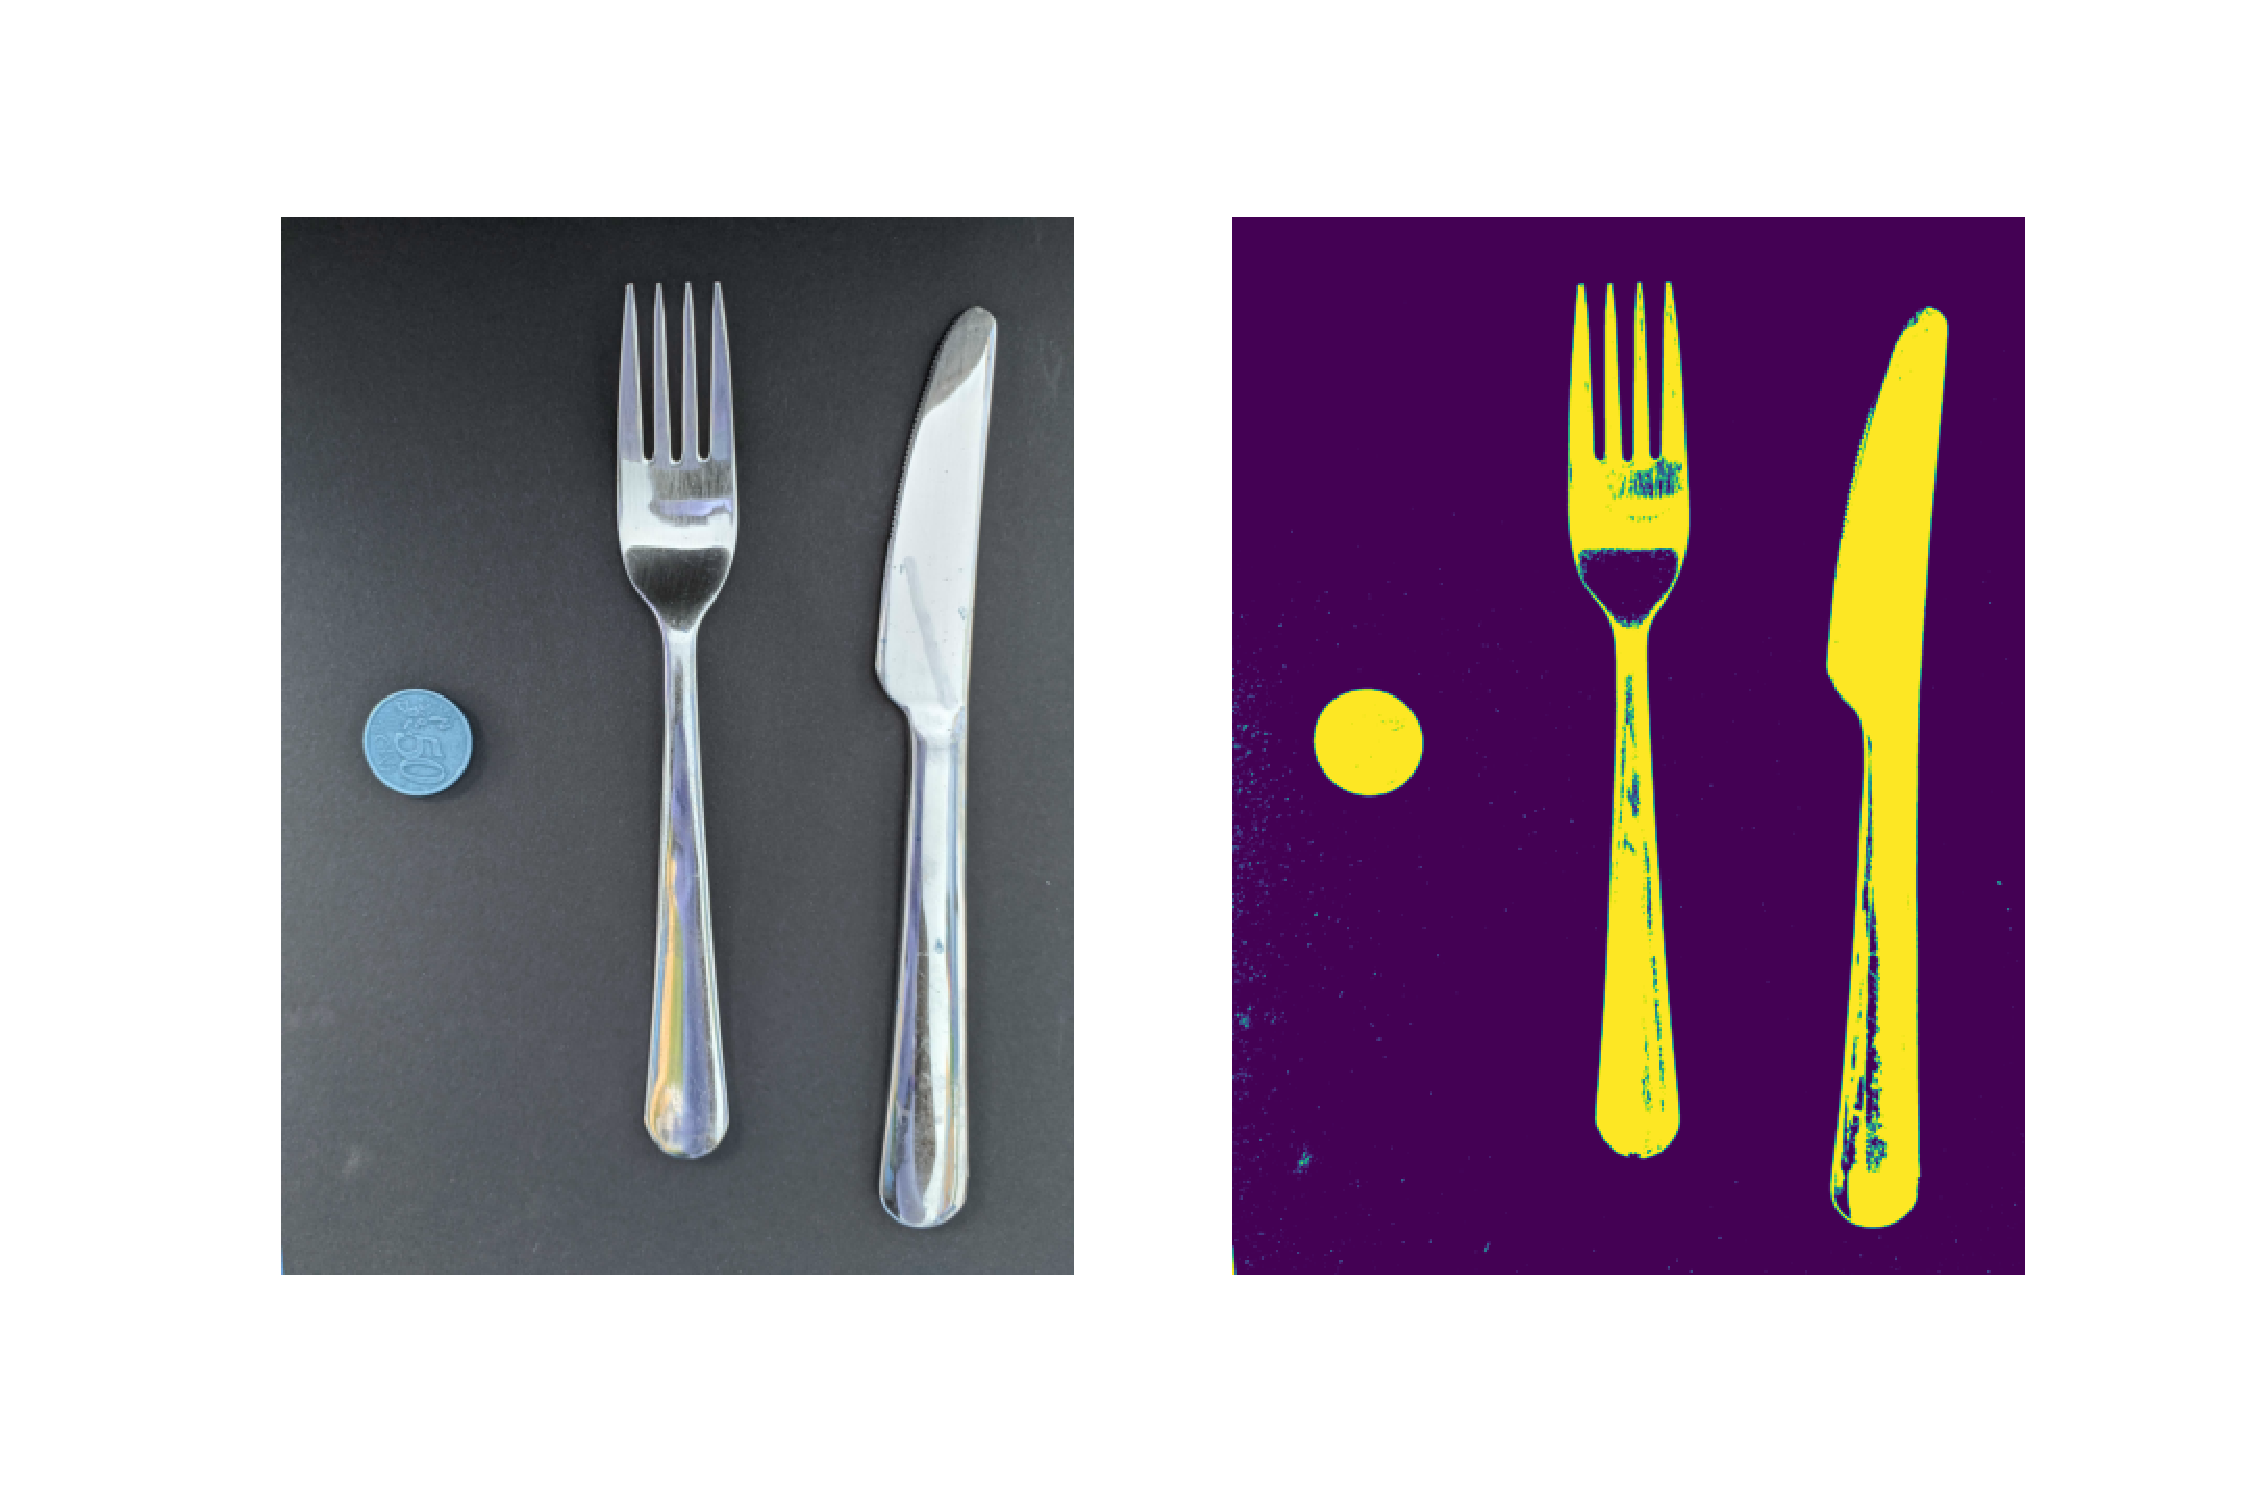
\includegraphics[scale=0.2]{binarization}
	\caption[center]{Umwandlung vom RGB- zum Binärbild}
	\label{fig:bin}
\end{figure}

Auf das Binärbild wurde anschließend ein Medianfilter angewandt um Rauschen aus dem Bild zu entfernen.

Das binarisierte und durch den Medianfilter bereinigte Bild wurde mit der Funktion findContours() anschließend nach Konturen abgesucht.

Um die Konturen herauszufiltern, die die Werkstücke am besten beschreiben muss in der Konfiguration des Skripts die Anzahl der auf dem Bild zu sehenden Objekte \{n\} angegeben werden. 
Somit können die \{n\} Flächenmäßig größten Konturen ausgewählt werden.

\section{Ergebnisse / Experimente}

\section{Ausblick}

\bibliographystyle{asmems4}

% Here's where you specify the bibliography database file.
% The full file name of the bibliography database for this
% article is asme2e.bib. The name for your database is up
% to you.
\bibliography{asme2e}

\end{document}
